% Copyright (c) 2017 Aleksa Sarai <asarai@suse.de>
% This work is licensed under the Creative Commons Attribution-ShareAlike 4.0
% International License. To view a copy of this license, visit
% http://creativecommons.org/licenses/by-sa/4.0/ or send a letter to Creative
% Commons, PO Box 1866, Mountain View, CA 94042, USA.

\documentclass[10pt,aspectratio=169]{beamer}
\usetheme{metropolis}
\metroset{background=light}
\metroset{titleformat=smallcaps}

\usepackage{pbox}
\usepackage{fontspec}
\usepackage[absolute,overlay]{textpos}
\usepackage[math-style=TeX]{unicode-math}
\usepackage{booktabs}

\usepackage{tikz}
\usetikzlibrary{calc}

\usepackage{hyperref}
\usepackage{graphicx}
\graphicspath{{.}{assets/}}

\usepackage{xcolor}
\definecolor{pPurple}{HTML}{EA00FF}
\definecolor{pRed}{HTML}{FF0000}
\definecolor{pOrange}{HTML}{EB811B}
\definecolor{pGreen}{HTML}{1E6A1E}

\setbeamertemplate{caption}{\raggedright\insertcaption\par}

\title{openQA}
\subtitle{Life is too short for manual testing!}
\author{%
		Aleksa Sarai \\
		Software Engineer \\
		SUSE Linux GmbH \\
		\href{mailto:asarai@suse.de}{\tiny\tt \underline{asarai@suse.de}}}

\date{}
\institute{}

\begin{document}
	\maketitle

	\begin{frame}{openQA?}
		\begin{itemize}
			\item Perl-based framework to ``emulate'' a user.
			\item Has support for:
			\begin{itemize}
				\item Running commands directly in a console.
				\item Emulating a keyboard.
				\item Emulating a mouse.
			\end{itemize}
			\item Uses ``needles'' to compare reference screenshots taken during a test.
		\end{itemize}
	\end{frame}

	\begin{frame}{What does it look like?}
		\begin{center}
			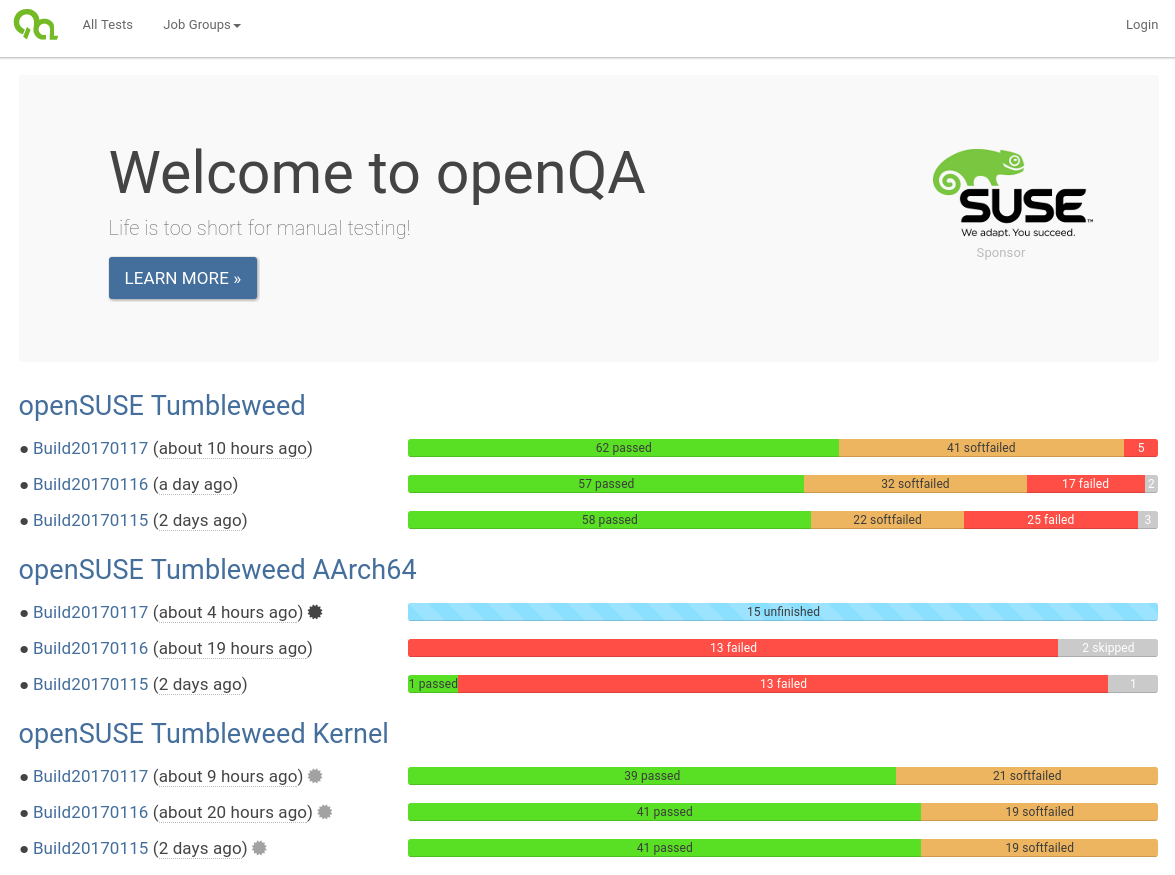
\includegraphics[height=0.7\textheight]{openqa_intro}
		\end{center}
		\begin{itemize}
			\item Used by openSUSE and SUSE to test distributions.
			\item \dots also starting to be used by Fedora.
		\end{itemize}
	\end{frame}

	\begin{frame}{``Needles''}
		\begin{itemize}
			\item OpenCV is used to compare reference ``needles''.
			\begin{itemize}
				\item It even has \textit{fuzzy} comparison!
				\item Console testing is just regular expressions.
			\end{itemize}
		\end{itemize}

		\begin{center}
			\only<1>{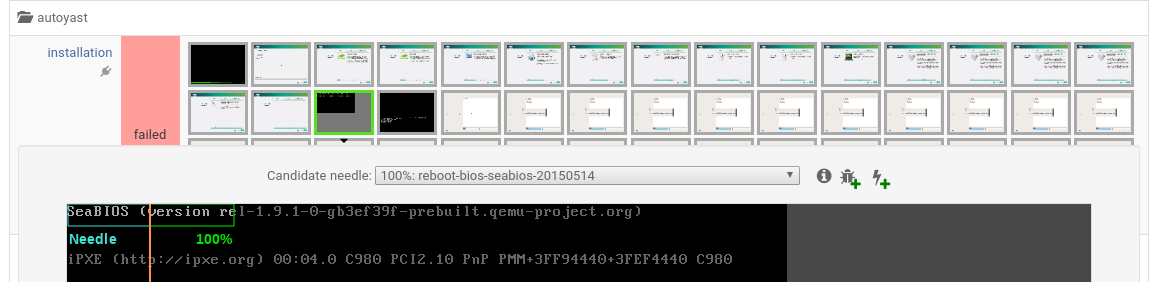
\includegraphics[width=0.8\textwidth]{openqa_needle_success}}
			\only<2>{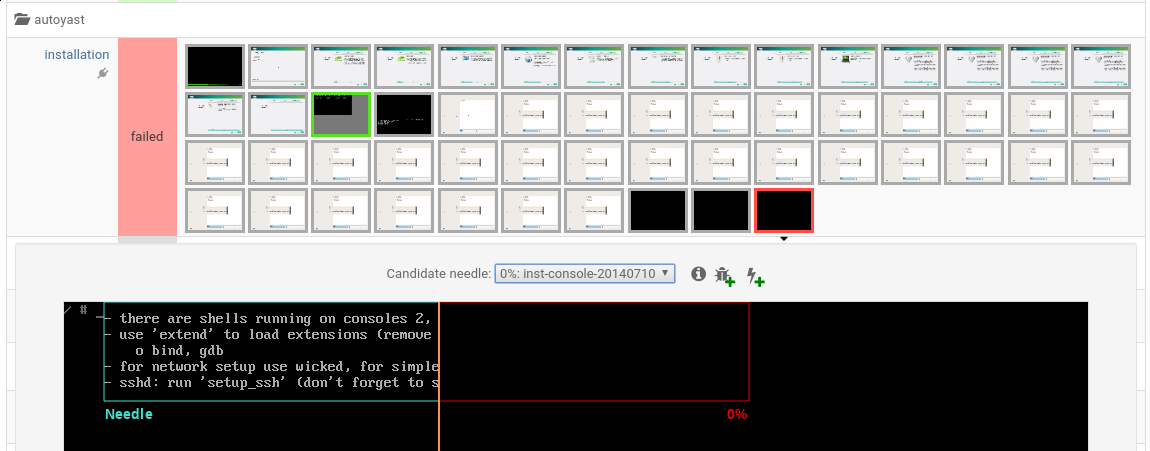
\includegraphics[width=0.8\textwidth]{openqa_needle_failure}}
		\end{center}
	\end{frame}

	\begin{frame}{Full Debuggability}
		\begin{itemize}
			\item All screen changes are stored in openQA for later debugging;
			\item \dots as are the VM disk images;
			\item \dots as are the source CDs used to create the environment.
		\end{itemize}

		\begin{center}
			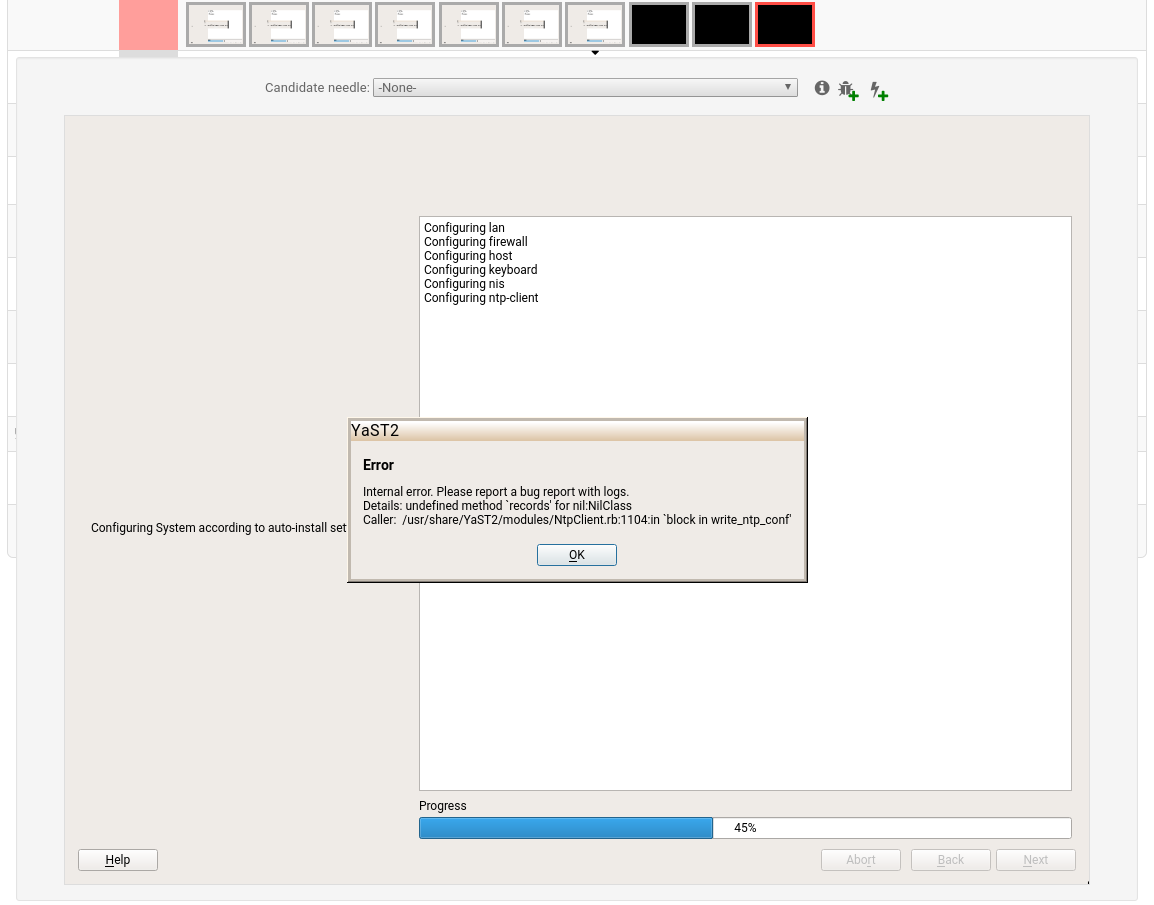
\includegraphics[height=0.7\textheight]{openqa_screenshot_prev}
		\end{center}
	\end{frame}

	\begin{frame}{Use it today!}
		\begin{itemize}
			\item If you're a distribution, QA testing is \textit{really} hard.
			\item \dots so start writing automated scripts!
			\item \url{http://open.qa/}
		\end{itemize}
	\end{frame}
\end{document}
